\subsection*{ Двумерное ДП, задача о рюкзаке [9]}
\begin{center}
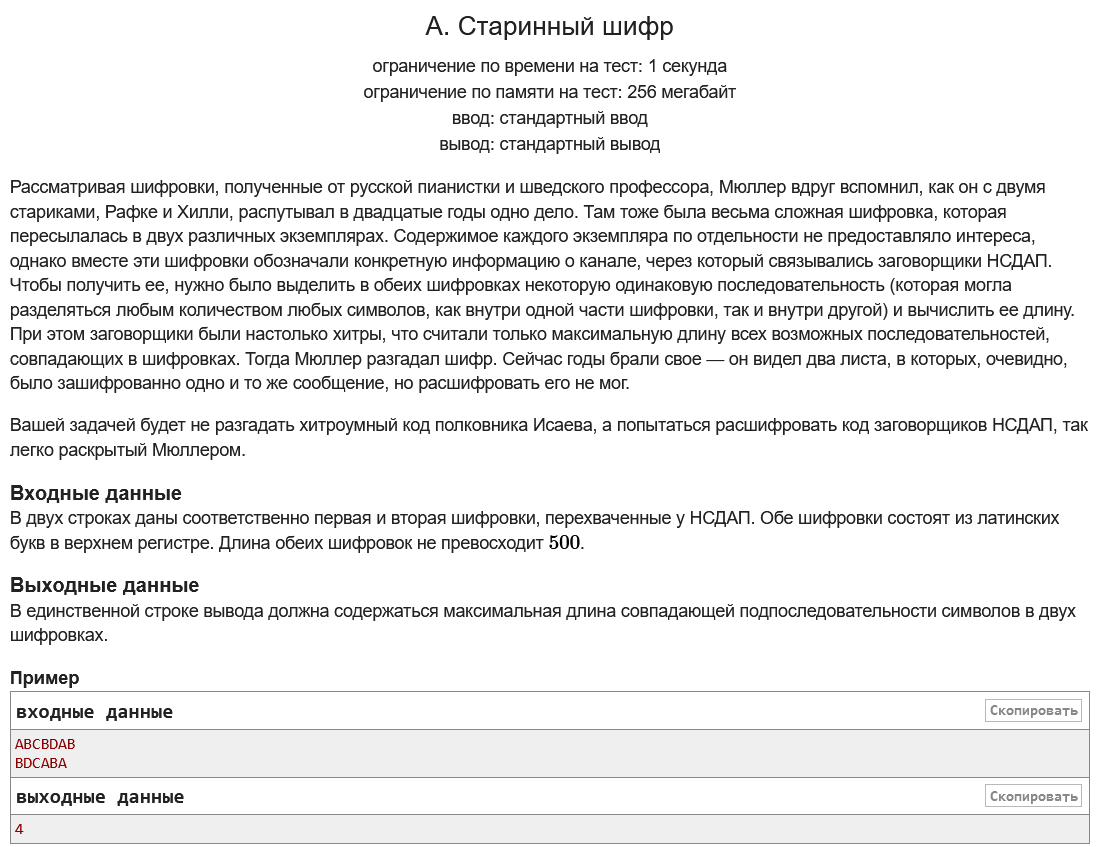
\includegraphics[width=\textwidth]{11A.png}
\end{center}
\subsubsection*{Идея решения}
Переборное решение будет работать за $O(n^2 * m^2)$, что при заданном условии не будет проходить ограничение по времени. При таком ограничении по времени зайдет только $O(n*m)$. Реализуем задачу о наибольшей общей возрастающей последовательности. $d[i][j]$ — это длина наибольшей общей возрастающей подпоследовательности префиксов $a[1..i]$ и $b[1..j]$, причем элемент $b[j]$ — последний представитель НОВП массива b, а $a[i]$ может не быть последним в массиве a. Вычислять d будем всё так же: сначала по увеличению i, а при равенстве — по увеличению j. Тогда для очередного значения $d[i][j]$ есть два варианта: 
\begin{itemize}
\item $a[i]$ не входит в НОВП. Тогда $d[i][j] = d[i-1][j]$: значение динамики уже посчитано на префиксе $a[1..i-1]$
\item $a[i]$ входит в НОВП. Это значит, что $a[i]=b[j]$, то есть для подсчёта $d[i][j]$ нужно пробегать циклом по b в поисках элемента $b[k]<b[j]$ с наибольшим значением $d[i-1][k]$. Но мы считаем d сначала по увеличению $i$, поэтому будем считать $a[i]$ фиксированным. Чтобы не запускать цикл при каждом равенстве $a[i]$ элементу $b[k]$, в дополнительной переменной best будем хранить "лучший" элемент (и его индекс ind в массиве b) такой, что этот элемент строго меньше $a[i]$ (а также меньше $b[k]$) и значение динамики для него максимально: $b[ind]<a[i]=b[j]$ и $best=d[i-1][ind] -> max$
\end{itemize}
\subsubsection*{Исходный код}
\begin{lstlisting}
#include <iostream>
#include <cmath>
#include <algorithm>
#include <vector>
#include <iomanip>
#include <unordered_map>
#include <unordered_set>
#include <map>
#include <set>
#include <string>
#include <stack>
#include <deque>

using namespace std;
typedef long long ll;

int main() {
    ios_base::sync_with_stdio(false);
    cin.tie(0);
    cout.tie(0);
    string a, b;
    cin >> a >> b;
    ll n = a.size(), m = b.size();
    vector<vector<ll>> dp(n + 1, vector<ll>(m + 1));
    for (int i = 1; i <= n; i++) {
        for (int j = 1; j <= m; j++) {
            if (a[i - 1] == b[j - 1]) {
                dp[i][j] = dp[i - 1][j - 1] + 1;
            }
            else {
                dp[i][j] = max(dp[i - 1][j], dp[i][j - 1]);
            }
        }
    }
    cout << dp[n][m];
    return 0;
}
\end{lstlisting}
\subsubsection*{Фрагмент турнирной таблицы контеста}
\begin{center}
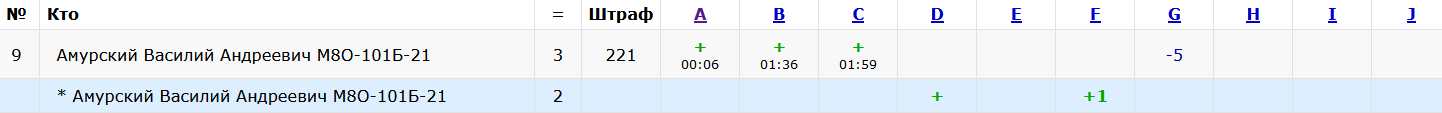
\includegraphics[width=\textwidth]{state11.png}\newline\noindent
\end{center}

\subsubsection*{Выводы}
Задача решена, проблем не возникло.
